\documentclass{article}
\usepackage[utf8]{inputenc}
\usepackage[a4paper, total={6in, 9.5in}]{geometry}
\usepackage{amsmath}
\usepackage{amssymb}
\usepackage{minted}
\usepackage{graphicx}

\graphicspath{{images/}}

\title{Sheet 10}
\author{Digdarshan Kunwar}
\date{November 2018}

\begin{document}
\maketitle
\section*{Problem 10.1}
\begin{minted}{C}
#include <unistd.h>
int main(int argc, char *argv[])
{
    for (; argc > 1; argc--) {
        if (0 == fork()) {
            (void) fork();  
        }
    }
    return 0;
}
\end{minted}
\textbf{a)}\\\\
\textbf{Case 1} ./foo, \\
$ argc = 1$  \\
$\bullet$ Parent process never loops\\
$\bullet$ There will be 0 child process as there is no loop \\

\texttt{Total Process :1 } 
\texttt{Child Processes:0}\\
\\
\textbf{Case 2} ./foo a,\\
$ argc = 2$\\
$\bullet$ The main process will be in the loop once\\
$\bullet$ The  child of main will never call the loop again,
and the  child will call fork() one time in the child process itself\\
$\bullet$ There will be 2 child processes in total \\

\texttt{Total Process :3 } 
\texttt{Child Processes:2}\\
\\
\textbf{Case 3} ./foo a b,\\ 
$ argc = 3$.\\
$\bullet$There will be 2 child process when $argc == 2$, which will have 3 process in total.\\
$\bullet$The main will also fork again if it loops.\\
$\bullet$In total, $ 3 * 3 = 9$ process, which means 8 child process . \\

\texttt{Total Process :9 } 
\texttt{Child Processes:8}\\
\\
We can observe in every iteration the number processes splits into 1 child and another sub child process.And if the child process is not the main parent(the first process) then it is also counted in the child process.So there will be 3 process in total in 1 iteration.\\
So we can relate it to a formula $Total Process=3^{n}$ for the total number of processes including the main parent process.\\
where $n$ is (argc-1).\texttt{(argc is argument count)}\\
Also the number of child processes can be written as $Total Process -1$\\\\
\textbf{Case 4} ./foo a b c, \\
$argc=4$\\
$\bullet$Here we have total of $3^{3}$ processes.\\
$\bullet$Excluding the main parent process we have 26 child process.\\

\texttt{Total Process :27 } 
\texttt{Child Processes:26}\\
\\
\textbf{Case 5}./foo a b c d, \\
$argc=4$\\
$\bullet$Here we have total of $3^{4}$ processes.\\
$\bullet$Excluding the main parent process we have 80 child process.\\

\texttt{Total Process :81 } 
\texttt{Child Processes:80}\\
\\
\subsection*{\textbf{b)}}
The code is given below : 
\begin{minted}{C}
#include <unistd.h>
#include <stdio.h>
#include <stdlib.h>

int main(int argc, char *argv[])
{
    for (; argc > 0; argc--) {
        int pid;
        pid=fork();
        if (pid == 0) { 
	  //delay the child process	
         	  sleep(10);
	  exit(1);
        }else{
	  //print the process id of childs
	  printf("The process id is : %d\n",pid); 
        }
    }
 
printf("\nThe main process ended\n\n");
return 0;
}

\end{minted}
Here the child or the zombie process is still running even if the parent process ends with the message.\\So we can see the zombie process with the top utility.Because they are still running the sleep() command in the process.\\
So they can be seen the the process list and we can check for their PID(Process Id).\\
The implementation is shown in the attached pictures as well.\\

\textbf{Creating zombie with different number of arguments :}\\
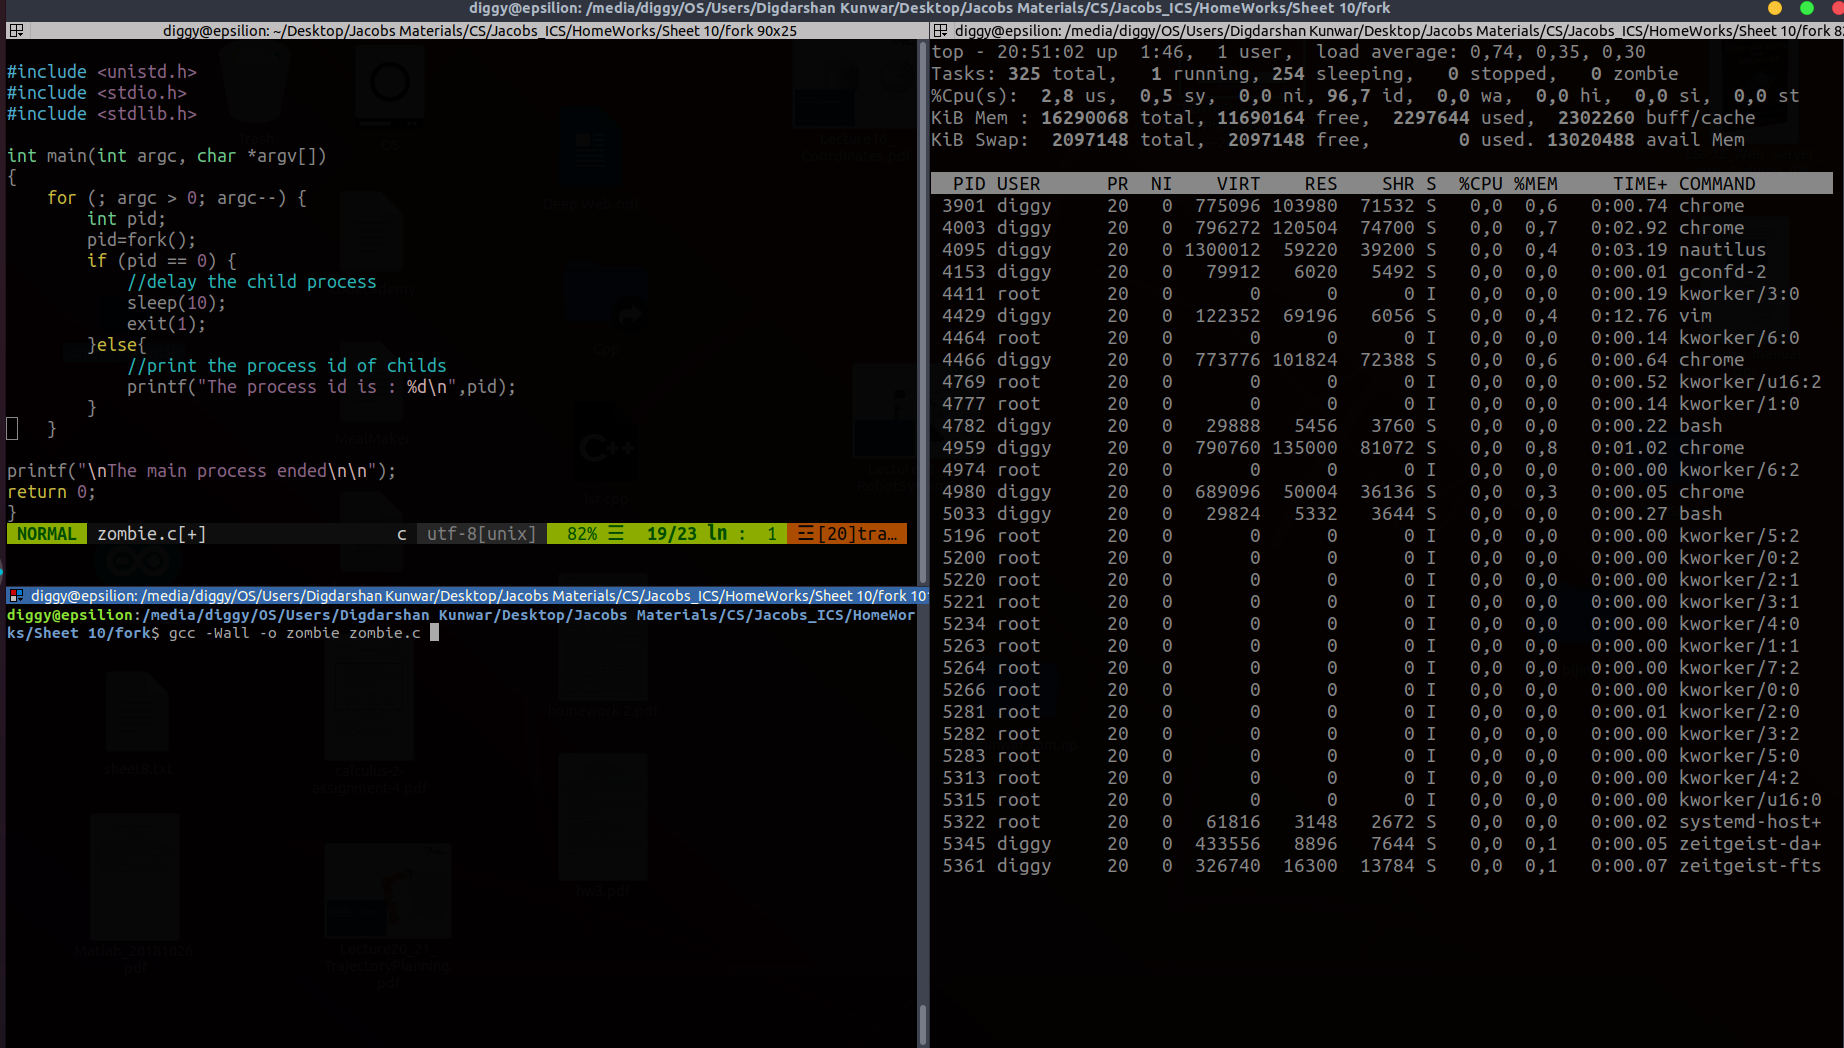
\includegraphics[scale=0.27]{image/1.png}\\
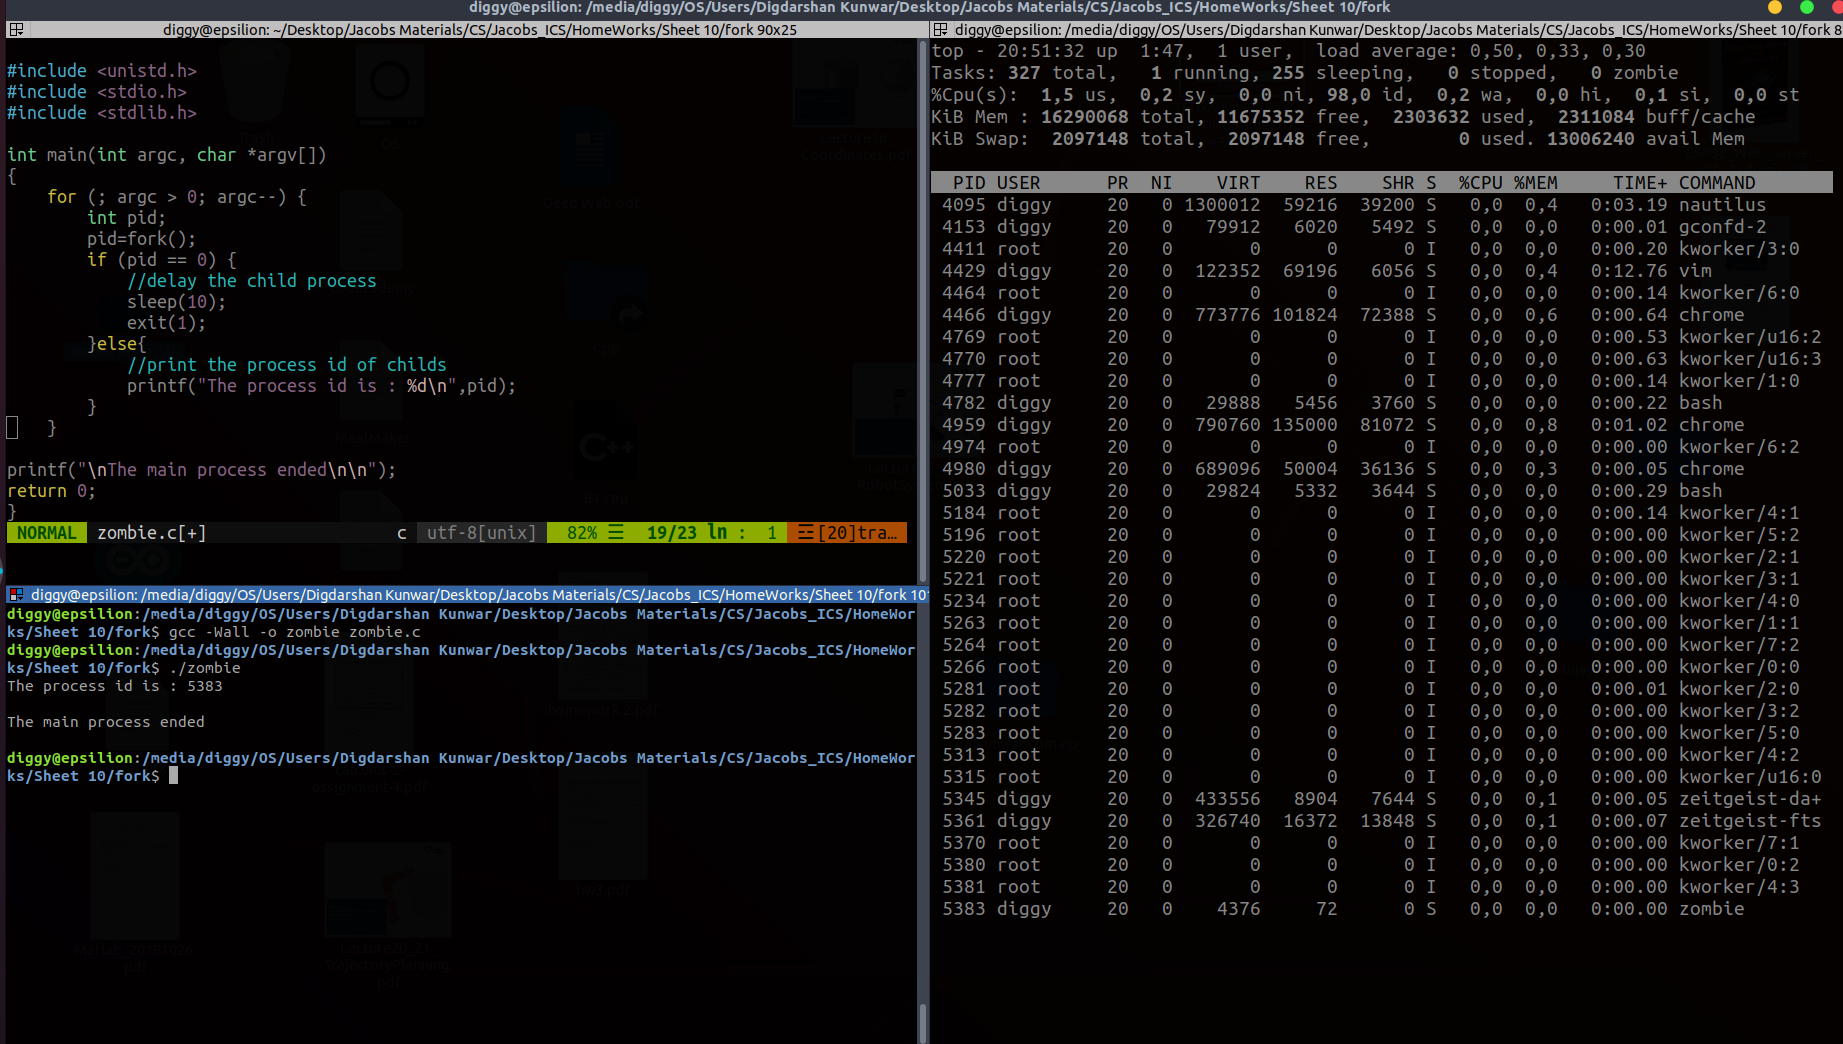
\includegraphics[scale=0.27]{image/2.png}\\
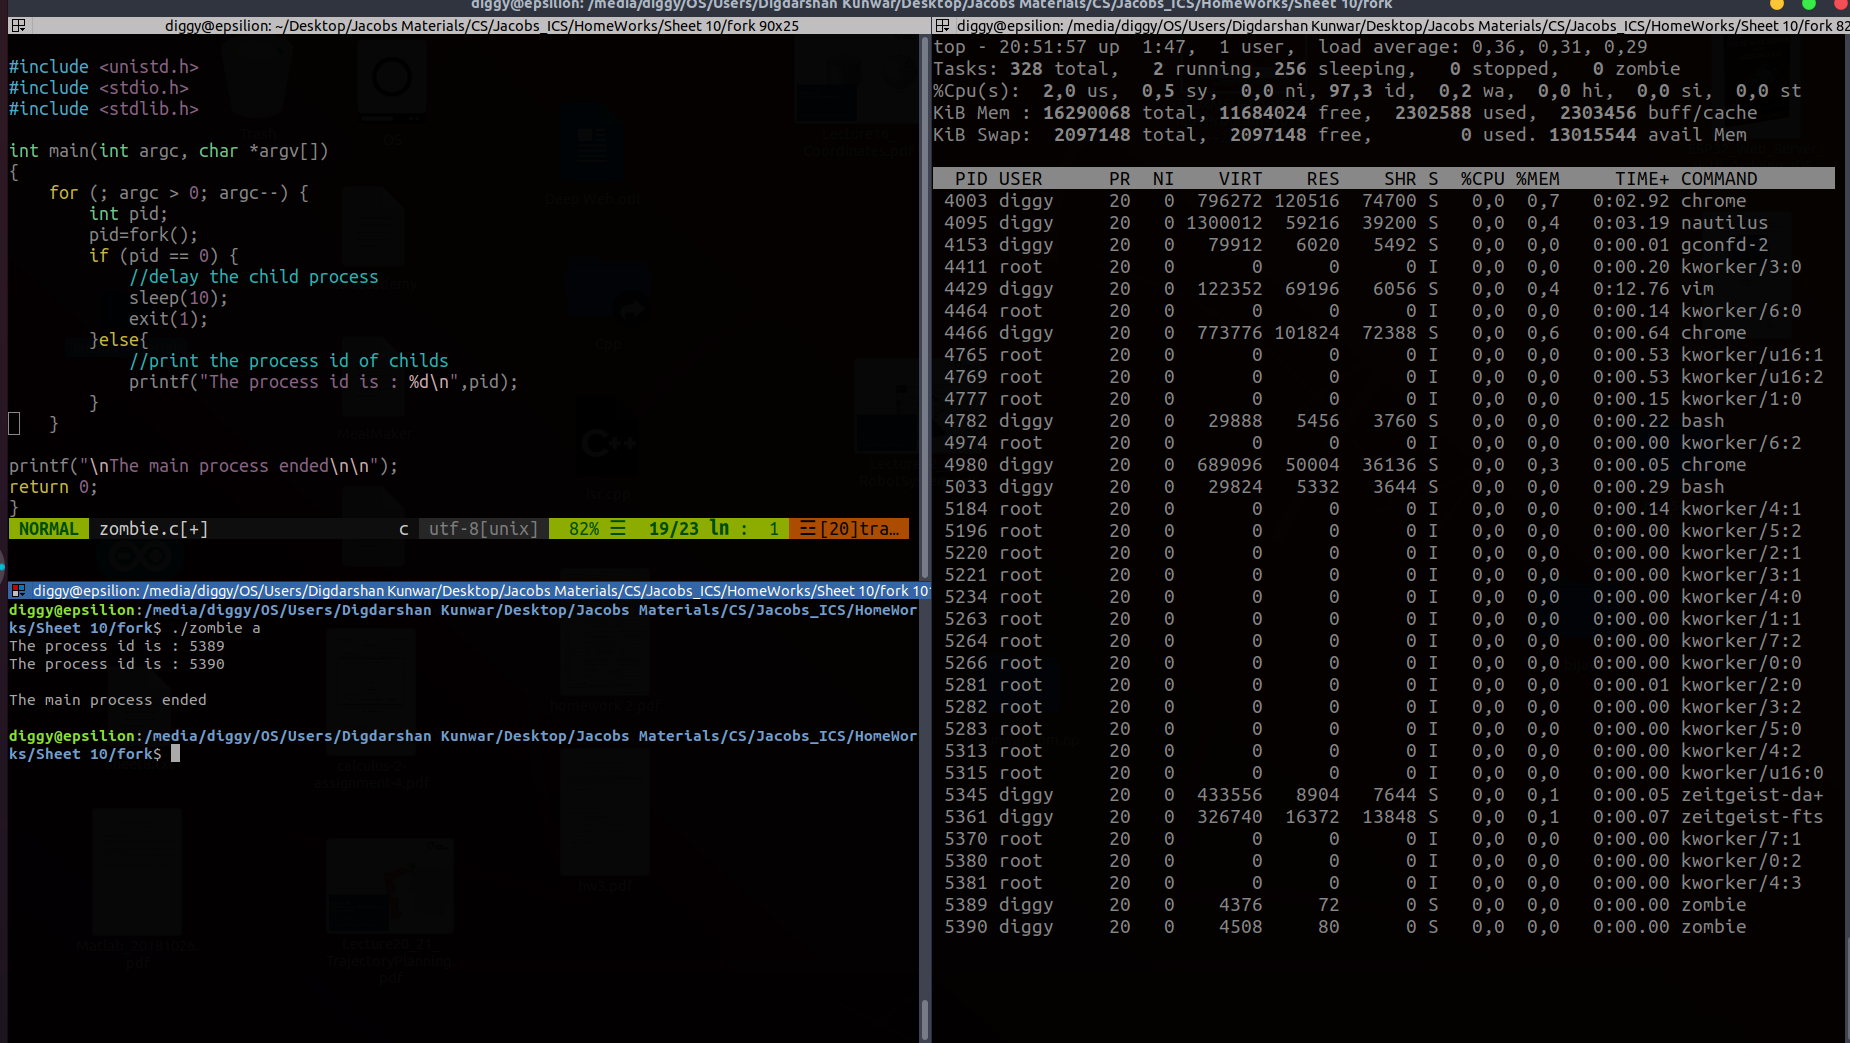
\includegraphics[scale=0.27]{image/3.png}\\
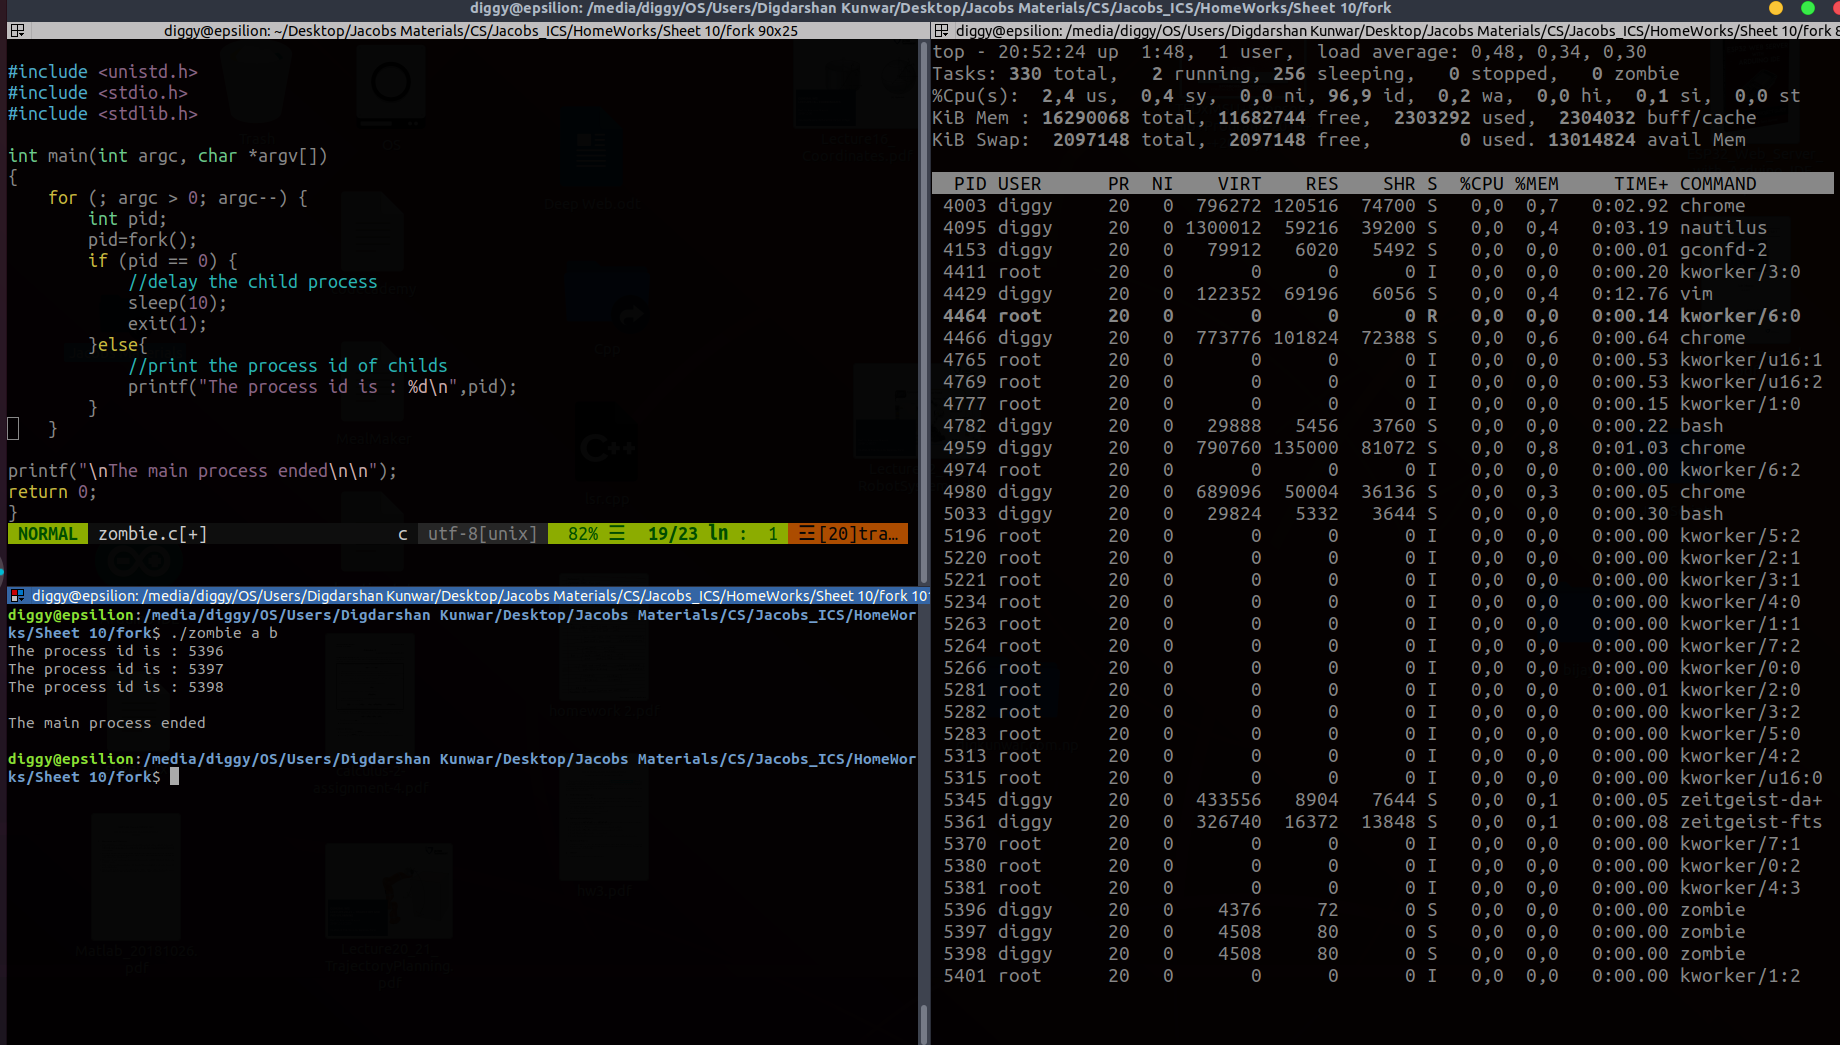
\includegraphics[scale=0.27]{image/4.png}\\
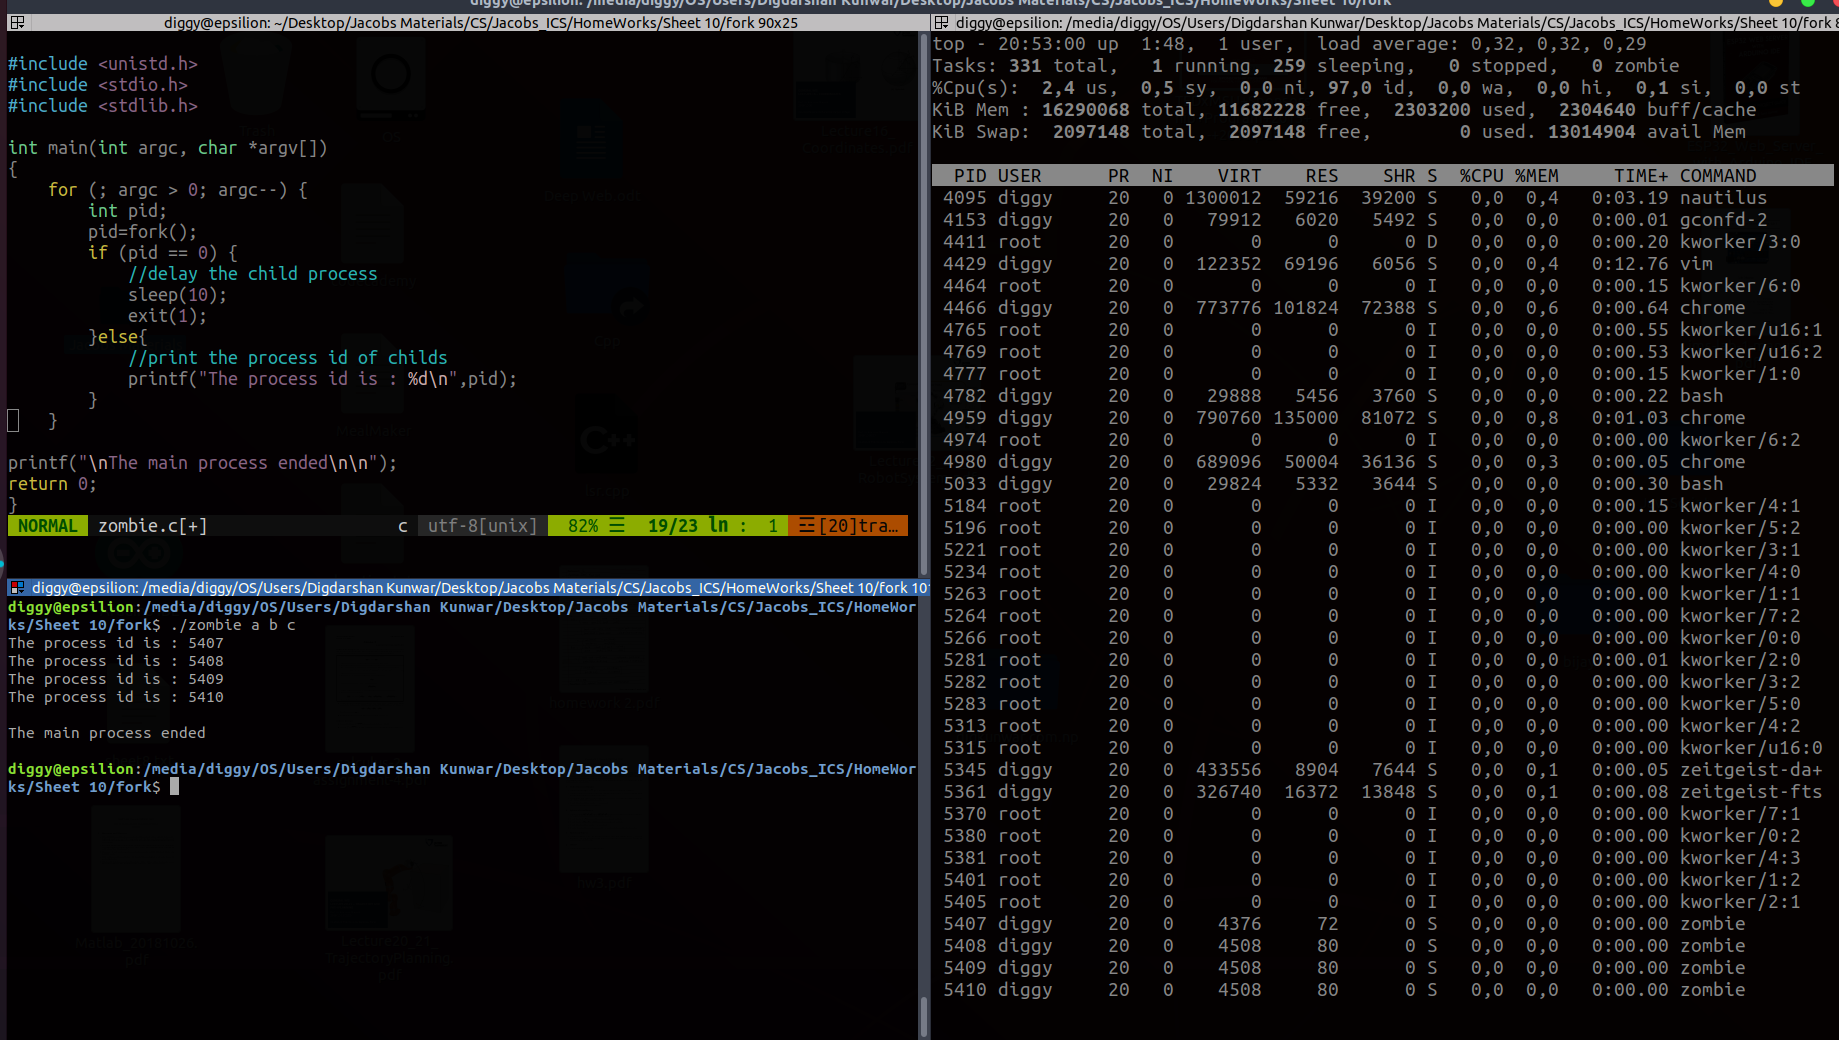
\includegraphics[scale=0.27]{image/5.png}\\


\noindent\rule{18cm}{0.4pt}
\section*{Problem 10.2}
The code is given below ::\\
\begin{minted}{C}
#include<iostream>
#include <dirent.h>
#include<string>
using namespace std;

/*
This program  recursively shows the content of the current working directory if no
arguments are passed to the main() function of the program. Otherwise, starts a
recursive listing for each of the arguments that are passed to the main() function.
*/

void search (char* name);
int main (int charc , char *charv[]) {
    char* root=new char[1]{'.'};
    if (charc==1){
        search(root);
        delete root;
         return 0;
    }else{
        //if the argc is more than 1
        for (int i =1;i<charc;i++){
            //Calling a search function in main   
            search(charv[i]);
        }
    }
    return 0;
}

//This is the search function 
void search (char* name){
    DIR *dir;
    char* fname;
    string loc,dirName;
    struct dirent *current;

    dir=opendir(name);

    //Check if the dir is NULL 
    if (dir!=NULL){
        
        while((current=readdir(dir))!=NULL ){
            //assign fname with the current->d_name
            fname=current->d_name;
            
            //if the file starts with . then neglect printing it 
            if (current->d_name[0] != '.'){

                if (name[0]=='.'&& name[1]=='\0'){
                    cout<<fname<<endl;
                    //location of contents (files) of that directory from current directory 
                    loc=fname;
                }else{
                    cout<<name<<"/"<<fname<<endl;
                    if (current->d_type== DT_DIR){
                        //Initial location of the file is name
                        loc=name;
                        //dirName is the filename of a file that is a directory
                        dirName=fname;
                        //loc is location of contents (files) of that directory from
                        current directory 
                        loc=loc+"/"+dirName;
                    }
                }
            }
            /*if the file is a directory then we have to read if that directory has
            other files in itself*/
            if (current->d_type== DT_DIR && current->d_name[0] != '.' ){

                //The below steps copy a string to a pointer 
                //Copies the loc to char pointer nloc
                char * nloc = new char[loc.size() + 1];
                copy(loc.begin(), loc.end(), nloc);
                nloc[loc.size()] = '\0';

                //Recusively go and read the files in directory
                search(nloc);   
                delete nloc;
            }
        }

    }else{
        //If the name doesnt match the directory or if dir is NULL
        cout<<"Error opening the Directory : "<<name<<endl;
    } 
    //Close the dir
    closedir(dir);
    }

\end{minted}


\end{document}
